\documentclass[12pt]{article}
% Defining all packages that are used in this document
\usepackage[utf8]{inputenc}
\usepackage[english]{babel} % Change this to norwegian if report is written in norwegian
\usepackage{amsmath}   % Package for math files
\usepackage{parskip}   % No indent, but instead paragraphs
\usepackage{graphicx}  % Place figures
\usepackage{caption}   % Place captions in tables and figures
\usepackage{subcaption}% 
\usepackage{subfiles}  % 
%\usepackage{subfigure}
\usepackage{pdfpages}
\usepackage[T1]{fontenc} 
\usepackage[euler]{textgreek} % To get greek letters as we know them
\usepackage{amssymb}   % 
\usepackage{placeins}  % \FloatBarrier so figures can't float beyond some point in text
\usepackage{fullpage}  % Uses more of the page
\usepackage{float}     % Able to make figures and tables float \begin{figure}[H] to keep them HERE
\usepackage[version=4]{mhchem} % \ce{} to write chemical eq.
\usepackage{siunitx}   % Ex: \si{\meter\per\square\second}
\usepackage{booktabs}  % Behind-the-scenes optimization of tables. \toprule, \midrule, \bottomrule
\usepackage{multirow}
\usepackage{hyperref}  % Ability to click on references like equations, figures, sections etc. \ref{eq:my_eq} clickable

%表格自动生成
\renewcommand {\thetable} {\thechapter{}.\arabic{table}}
%表格根据章节自动命名
\renewcommand {\thefigure} {\thechapter{}.\arabic{figure}}
%图片根据章节自动命名
\numberwithin{figure}{section}
\numberwithin{table}{section}
\numberwithin{equation}{section}
%以上三个皆控制重命名

\usepackage{fontspec}
\setmainfont{Arial}

\hypersetup{
    colorlinks,
    citecolor=black,
    filecolor=black,
    linkcolor=black,
    urlcolor=black
}
\iffalse
\usepackage{fancyhdr}
	%fancyhdr:一个很强大的宏包,用于自定义设计页面风格并命名以供调用。
	\pagestyle{fancy}
	%\rhead{实验B16 基于vLight的光学仿真基础实验}
	%\lhead{基础物理实验\uppercase\expandafter{\romannumeral2}实验报告}
	\cfoot{ \thepage}  %当前页
	\rfoot{\today}
		%分别是右页眉、左页眉、中页脚、右页脚
	\renewcommand{\headrulewidth}{0pt}
	%\renewcommand{\theenumi}{(\arabic{enumi})}
\fi

\usepackage[autolinebreaks,useliterate,numbered]{mcode} % Ability to paste smooth MATLAB code
\newcommand{\figref}[1]{\figurename~\ref{#1}} %Nice reference to figures
%\linespread{1}
\usepackage{setspace}
\setstretch{1}
%\renewcommand{\baselinestretch}{1.5}
\title{
    Plastic Collapse of Portal Frame Lab  \\
    Group T05
    }
\author{
	Jiaqi, Yao.%\footnote{jy431@exeter.ac.uk}
}
\date{
    \today
}

\begin{document}
\maketitle
%\begin{abstract}
%    This section should contain a short and concise way of describing all parts of the report. It should be a summary of the introduction, what has been done and what you have found.
%\end{abstract}
\pagenumbering{gobble} % Turn off page numbering
%\newpage
%\tableofcontents
%\newpage
\pagenumbering{arabic} % Turn on normal pagenumbering
%%%%%%%%%%%%%%%%%%%%%%%%%%%%%%%%%%%%%%%%%%%%%%%%%%%%%%%%%%
% Main contents - Do NOT write your text in main.tex! Use                     the tex files in the folders below
\section{Brief report}

	\noindent Dear Officer:
	
	\noindent We understand that you are looking for a welding robot for the automotive industry and our team has found our product to be the right fit for your needs. I will then briefly describe our robot and show its advantages in terms of design and precision.
	
	\noindent We have designed a four-armed robot according to your requirements and have considered its parameters, which you can see in Table 1 and Table 2. After simulation analysis, this design is reasonable and can perform the task accurately in the working area. We have also created a kinematic diagram (Figure 2.1) and a workspace diagram (Figure 3.1)
	
	\noindent The maximum error in end effector position on the x and z axes is below 0.05, while the maximum error on the y axis is slightly This shows the amazing accuracy of the robot in its movements and workings. You can see the specific images of the errors in Figure 1 and Figure 2.

\section{Introduction}
\FloatBarrier % Now figures cannot float above section title

Our product is a type of mechanical equipment used for automated welding. Our robotic arm can be widely used in various welding operations in the manufacturing industry, including automotive manufacturing, aerospace, construction, and manufacturing.

Our product has many adavantages. Firstly, it can improve production efficiency and quality by reducing the negative impact of human factors on production through automated welding operations. Secondly, it can reduce the danger of the work environment. 

In summary, the four-arm welding robot is an efficient and accurate welding device with many advantages. It will become an important part of automated production in the manufacturing industry, providing a reliable solution for various production operations.









\iffalse
The purpose of this experiment is to investigate the behaviour of a mild steel portal frame model when subjected to increasing loads.

The rig consists of a loading system that applies a vertical load at the center of the beam and a horizontal load at the top of one column. As shown in \autoref{f0}.

\begin{figure}[htbp]
    \centering
    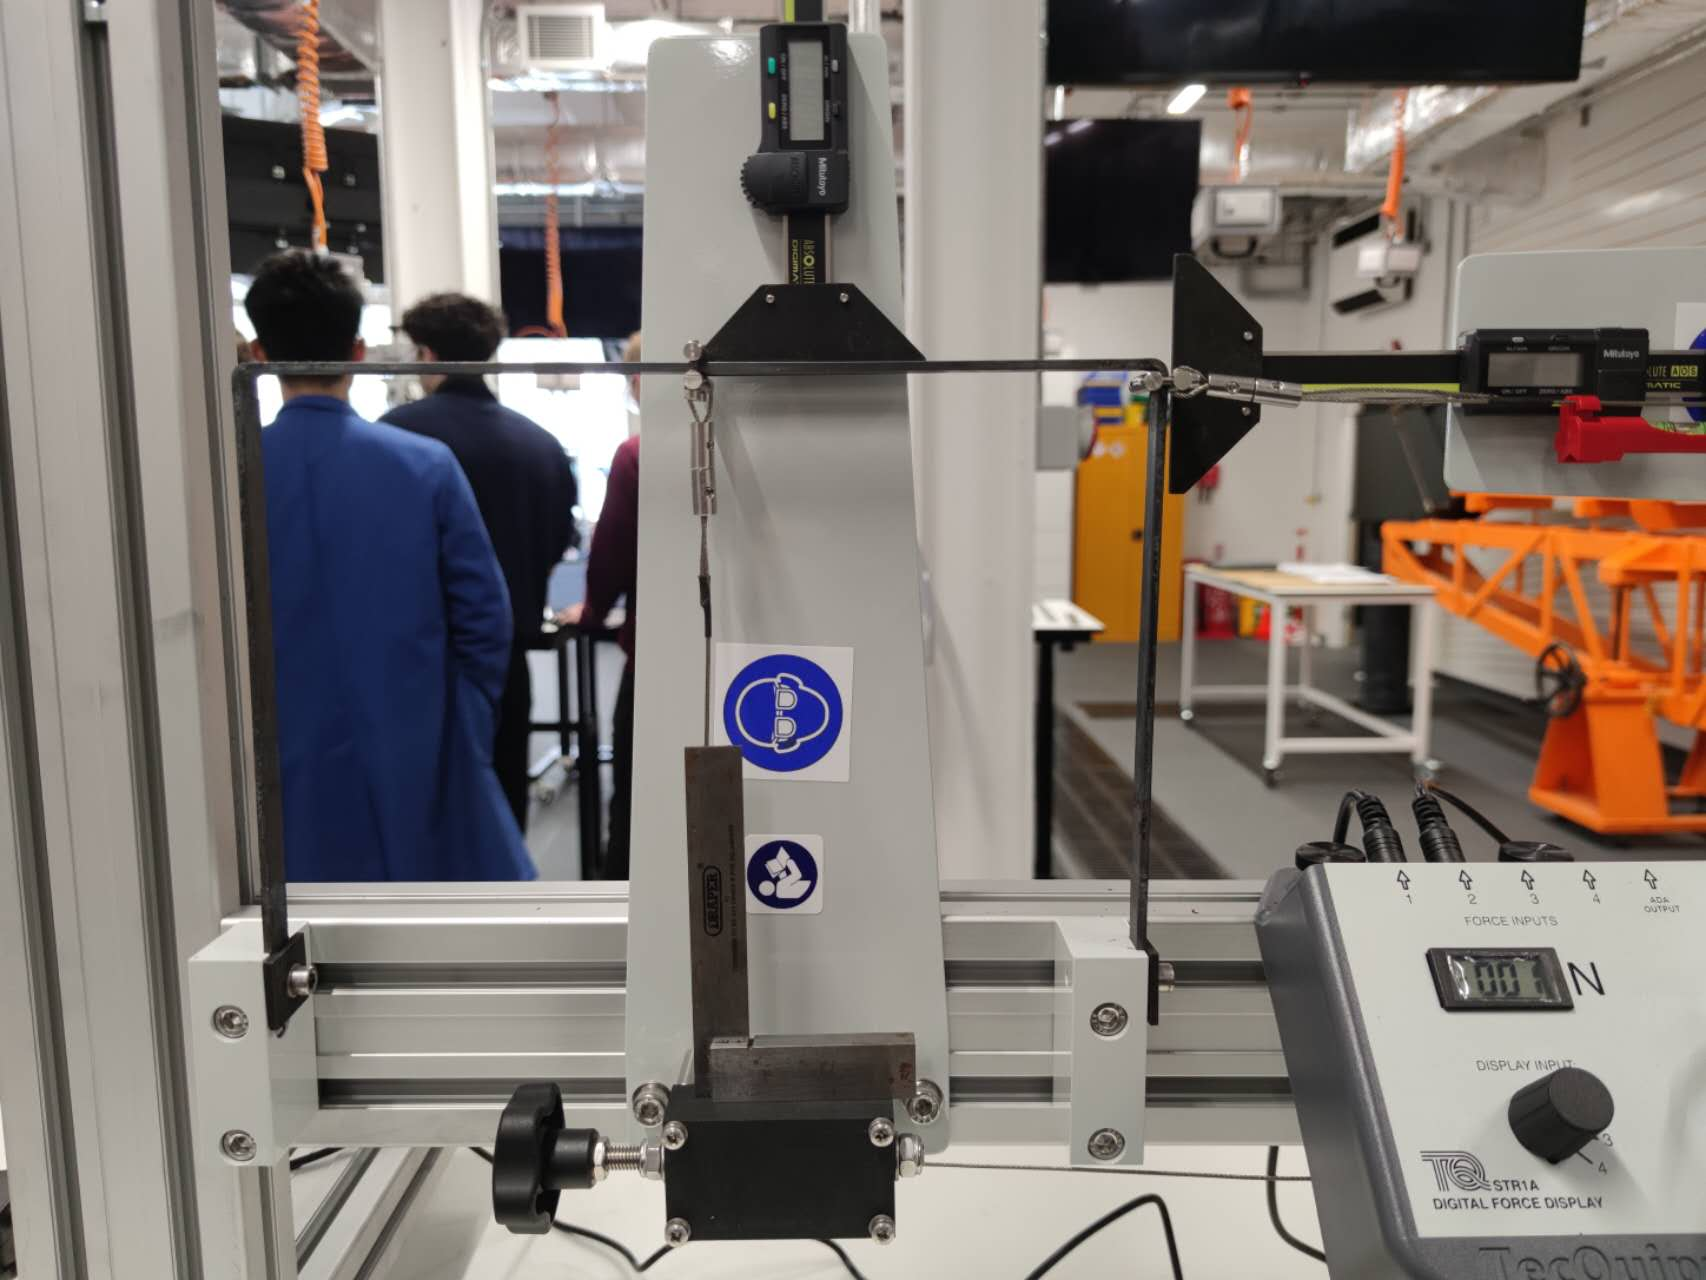
\includegraphics[width=7.5cm]{./fig/00.jpg}
    \caption{Experimental procedure}
    \label{f0}
\end{figure}

\fi



\section{Experiment}
\FloatBarrier % Now figures cannot float above section title

The frame is made of mild steel and has a uniform rectangular cross-section. Also, The rig is equipped with two gauges to monitor the horizontal deflection of the beam and its central vertical deflection. The yield strenth of the steel is 250MPa.

The experimental parameters are shown in the following table \autoref{t1}.

\begin{minipage}[htbp]{\textwidth}
    \makeatletter\def\@captype{table}
    \centering
    \scalebox{1}{
        \begin{tabular}{lllll}
            \hline
            Data type &Height & Length & Thickness & Width \\ \hline
            Theory&200    & 300    & 3.00      & 12.00 \\ 
            Actual&200    & 304    & 3.27      & 12.97 \\ \hline
            \end{tabular}} 

    (Unit: mm)
    \caption{Experiment parameters}
    \label{t1} 
\end{minipage}


The experiment entails the following steps:
\begin{enumerate}
    \item Measure and record the dimensions of the frame and its cross-section.

    \item Ensure the loading rig is in proper working condition and inspect cables for damage.
    
    \item Zero the force and displacement readings while the rig is still unloaded.
    
    \item Gradually apply increasing horizontal and vertical loads to the frame in increments of 10 N. The relationships between P and W are $y=x$\label{ee1}.
    
    \item Record the applied forces and corresponding deflections for each increment.
    
    \item Continue the process until a plastic failure occurs, and observe the formation of plastic hinges and position.
    
    \item Unload the frame and identify the locations of plastic hinges by observing permanent rotation in the joints.
    
\end{enumerate}

Here are the recorded data \autoref{t2}.

\begin{minipage}[htbp]{\textwidth}
    \makeatletter\def\@captype{table}
    \centering
    \scalebox{0.85}{
        \begin{tabular}{ccccccccccccccc}
            \hline
            \multirow{2}{*}{Force(N)}    & Vertical   & 10   & 20   & 30   & 40   & 50   & 60   & 70   & 80   & 90   & 100  & 110  & 120   & 130   \\
                                      & Horizontal & 10   & 20   & 30   & 40   & 50   & 60   & 70   & 80   & 90   & 100  & 110  & 120   & 130   \\ \hline
            \multirow{2}{*}{Distance(mm)} & Vertical   & 0.06 & 0.05 & 0.1  & 1.42 & 2.13 & 2.26 & 2.8  & 3.22 & 3.62 & 4.28 & 5.23 & 7.46  & 12.88 \\
                                      & Horizontal & 0.88 & 1.58 & 2.15 & 2.99 & 4.04 & 4.44 & 5.06 & 6.48 & 7.63 & 8.55 & 9.31 & 15.05 & 23.08 \\ \hline
            \end{tabular}} 
    \caption{Record data}
    \label{t2} 
\end{minipage}

\section{Theory}
\FloatBarrier % Now figures cannot float above section title

The method of calculating the plastic moment is introduced in the powerpoint of the Week 6 lecture. As shown in the figure below \autoref{f1}.

\begin{figure}
    \centering
    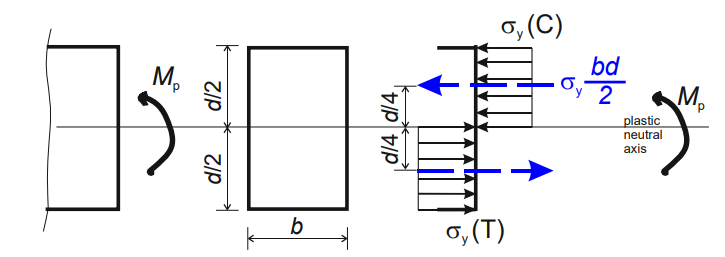
\includegraphics[width=10cm]{./fig/11.png}
    \caption{plastic modules of rectangular section  }
    \label{f1}
\end{figure}

The plastic moment $M_p$ when all points in the section reached
yield stress $\sigma_y(250Mpa)$ is caculated by:

\begin{equation} 
    M_p=\sigma_y\frac{bd}{2}(\frac{d}{4}+\frac{d}{4})
    \label{e1}
\end{equation}

Calculated from the data from \autoref{t1}, we get $M_p=8.67N \cdot m$.

There are three cases of collapse of plasticity of portal frame. We use virtual work method to caculate it.

\begin{figure}[htbp]
    \centering
    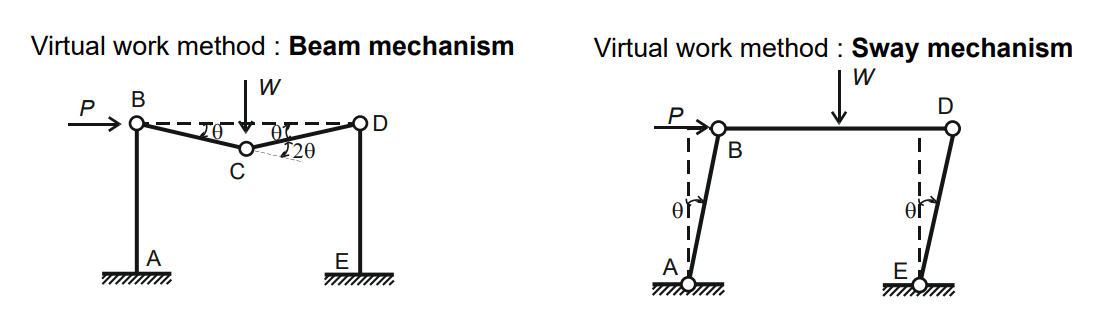
\includegraphics[width=10cm]{./fig/12.png}
    %\caption{plastic modules of rectangular section  }
    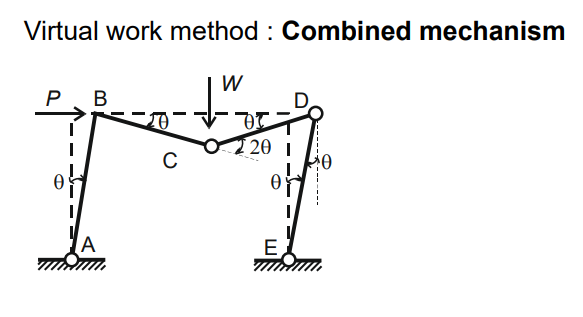
\includegraphics[width=5.5cm]{./fig/13.png}
    \caption{Three cases of collapse of plasticity of portal frame}
    \label{f2}
\end{figure}


$\bullet$ \textbf{Beam mechanism:} If $W>>P$, the hinges are likely to appear in B, C and D.



$\bullet$ \textbf{Sway mechanism:} If $P>>W$, the hinges are likely to appear in A, B, D and E.




$\bullet$ \textbf{Combined mechanism:} If P $\approx$ W, the smallest moment
is at B (as moments due to P
and W oppose each other), so
hinges form at other possible
locations. (The angle between ABC is $90^\circ$)

The virtual work method is: 

\begin{equation}
    \sum_i^{}{P_i\delta_i}=\sum_j^{}{M_j\theta_j}
    \label{e2}
\end{equation}

We noticed that the height (200mm) is equal to $\frac{2}{3}$ length (300mm). i.e. $H=\frac{2}{3}L$.

By using \autoref{e2}, we can get

$$
\left\{ \begin{array}{l}
	W\frac{\theta L}{2}=M_p\theta+M_p2\theta+M_p\theta \rightarrow W=\frac{8M_p}{L} (Beam)\\
	P\frac{2L}{3}\theta=M_p\theta+M_p\theta+M_p\theta+M_p\theta \rightarrow P=\frac{6M_p}{L} (Sway)\\
	P\frac{2L}{3}\theta+W\frac{\theta L}{2}=M_p\theta+M_p2\theta+M_p2\theta+M_p\theta \rightarrow 4P+3W=\frac{36M_p}{L} (Combined)\\
\end{array} \right. 
$$

Plot the relationships P-W on a graph

\begin{figure}[htbp]
    \centering
    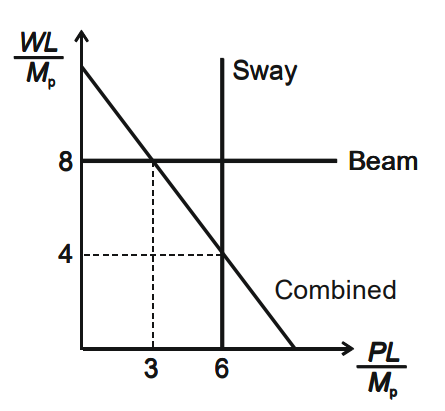
\includegraphics[width=6.5cm]{./fig/14.png}
    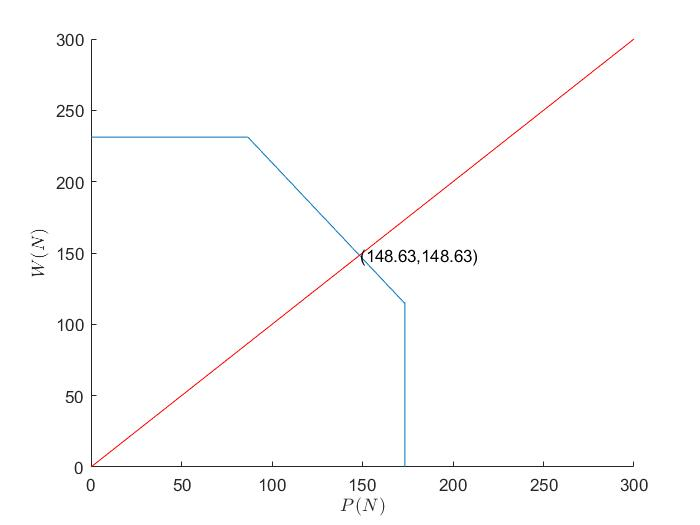
\includegraphics[width=8.5cm]{./fig/15.jpg}
    \caption{P-W graph}
    \label{f3}
\end{figure}



Substitude data from \autoref{t1} and \autoref{e1}, We have $\frac{M_p}{L}=28.9N$ and the boundary of the graph.

$$
\left\{ \begin{array}{l}
	W=\frac{8M_p}{L}=231.2\\
	P=\frac{6M_p}{L}=173.4\\
	4P+3W=\frac{36M_p}{L}=1040.4\\
\end{array} \right. 
$$

Plotting the three boundary lines with the applied load lines ($y=x$) on the graph, the following figure is obtained.

$$
\left\{ \begin{array}{l}
	4P+3W=1040.4\\
	P=W\\
\end{array} \right. 
$$
The solution to the equation is ($P=W=148.63(N)$)
where the coordinates of the load line and the boundary line are (148.63,148.63\label{ee}).








\section{Analysis}
\FloatBarrier % Now figures cannot float above section title

\subsection*{A : presentation of force vs deformation relationships}
Using the data in Table 2, the force vs deformation plot can be derived as \autoref{f3}. Also, from the lecture in week 7, we can learn that the total bending moment diagram is as follows


\begin{figure}[htbp]
    \centering
    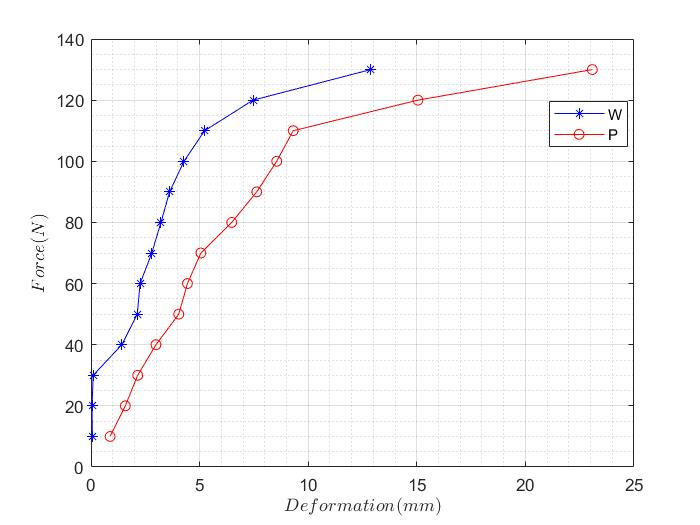
\includegraphics[width=9cm]{./fig/17.jpg}
    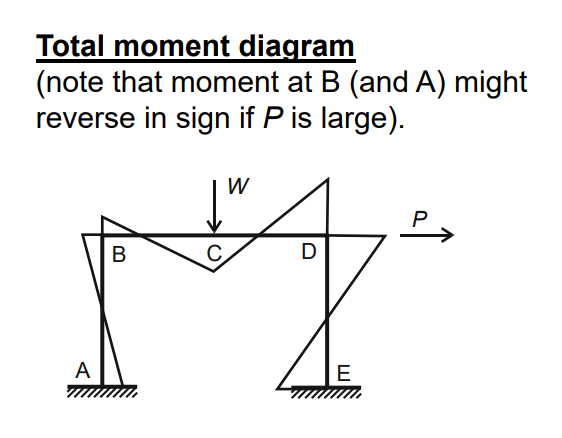
\includegraphics[width=7cm]{./fig/16.png}
    \caption{Force vs deformation and total moment diagram}
    \label{f4}
\end{figure}


The chart illustrates the relationship between the strength and deformation of steel, which can be discussed in two different situation.

$\bullet$ W<110N,P<110N: Elastic deformation: The relationship between the elastic deformation variable and the external force is linear.

$\bullet$ W$\geq$110N,P$\geq$110N: Plastic deformation: The relationship between force and deformation is nonlinear, i.e., the strain shows a rapid increase with the increase of stress.

From the overall bending moment diagram (see \autoref{f4}), it can be seen that point D has the maximum bending moment, making it the first point in the experiment to experience plastic deformation.

In \autoref{f3}, The P-W graph is piecewise and if the combination of the P and W exceeds the closed figure on the left, The collapse will happen. In this case$(y=x)$, the collapse load for the frame was $W=148.63N,P=148.63N(Theoretical)$.

Based on the \autoref{f4} (ignoring the inaccurate data at the beginning), it can be analyzed that the first plastic hinge is formed at around 110 N, where a significant change can be observed in the slope of the W curve. The remaining plastic hinges are formed at around 120 N, where both the P and W segments exhibit drastic changes.

%\textit{Can you identify at which load each plastic hinge formed?}


\subsection*{B : explaination of plastic hinges}

\begin{figure}[htbp]
    \centering
    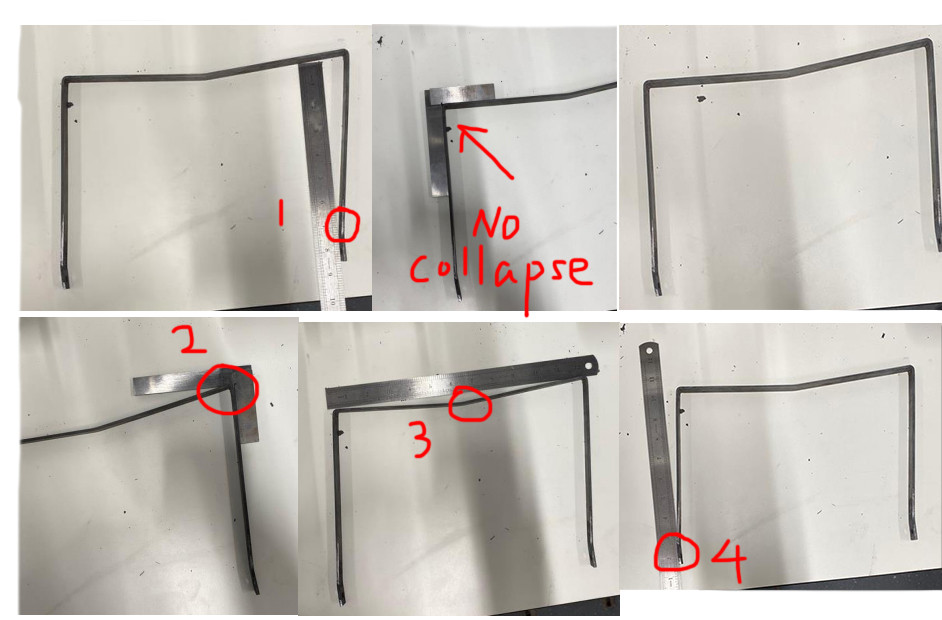
\includegraphics[width=10cm]{./fig/18.jpg}
    \caption{Experimental results}
    \label{f5}
\end{figure}

There are 4 plastic hinges at the moment of the collapse of the frame. Compare \autoref{f2} and \autoref{f5} we can find: 

$\bullet$ After the force load, the upper left corner of the frame did not rotate, and the angle between the beam and column was still degrees.

$\bullet$ The angle of rotation of the plastic collapse occurring at points 1,4 is $\theta$(in \autoref{f2}).

$\bullet$ The angle of rotation of the plastic collapse occurring at points 2,3 is $2\theta$(in \autoref{f2}), which is double that of points 1,4.

\subsection*{C : compare the theoretical and actual}
\subsubsection*{i}

The theoretical plastic collapse load derived from Section 2 is 148.63N, while the actual collapse load is in the region of $110N$-$120N$.($23.8\%$)

The comparison leads to the conclusion that the actual collapse load will be less than the theoretical value for these possible reasons:

$\bullet$ \textbf{Geometric discrepancies:} The actual dimensions of the frame may differ from the theoretical dimensions, as seen in \autoref{t1}. These discrepancies may affect the frame's overall stiffness and load-carrying capacity.(theoretical $M_p=6.75N$ vs actual $M_p=8.67N$)

$\bullet$ \textbf{Material imperfections:} The mild steel used in the experiment may contain imperfections like inclusions, voids, or uneven distribution of constituents, which could affect its mechanical properties and reduce its strength.

$\bullet$ \textbf{Load application:} The loading rig's accuracy in applying the horizontal and vertical loads may impact the results. Inaccurate load distribution or misalignment could cause the frame to experience additional stresses, leading to a reduced collapse load.

$\bullet$ \textbf{Measurement errors:} The gauges used to monitor the deflection of the frame might have inaccuracies, leading to discrepancies between the actual and recorded deflections.

\subsubsection*{ii}

$\bullet$ There are 4 plastic hinges in theory (\autoref{f2}-Combined mechanism). The positions of the plastic hinges are points A, C, D and E.

$\bullet$ There are 4 plastic hinges in experiment (\autoref{f5}). The positions of the plastic hinges are in the position 1,2,3,4.

$\bullet$ Compared with that, it is easy to see that the theoretical and actual positions of the plastic hinges are roughly the same.

\subsubsection*{iii}

The overall shape of the measured and predicted collapse mechanism are same. In \autoref{f2} and \autoref{f5}, the upper left corner is not deformed, a rotation of angle $\theta$ occurs at positions 1,4 and a rotation of angle $2\theta$ occurs at positions 2,3.
\section{Conclusion}

In conclusion, we successfully built the four-arm robot and achieve the function of welding in a specific area. We designed all the relevant data and reduced the errors by simulink. The maximum error in end effector position on the x and z axes is below 0.05, while the maximum error on the y axis is slightly over 0.10, and the largest error of joint angle is joint2 angle, and it just nearly reaches 0.02. These errors are far better than the standards set. Overall, we achieved the desired results. This is certainly a product worth buying and will bring unimaginable benefits to your company

%\section*{List of Symbols}
\begin{table}[H]
\centering
\begin{tabular}{lll}
 \toprule
  \textbf{Symbol}   &\textbf{Unit}      &\textbf{Explanation}\\
  \midrule
    n               & \si{\mole}        & Amount of substance \\
    m               & \si{\kilo\gram}   & Mass \\
    H               & \si{\kilo\joule\per\mole} & Molar enthalpy \\
    S               & \si{\joule\per\kelvin\per\mole}   & Molar entropy \\
    G               & \si{\kilo\joule\per\mole} & Gibbs free energy \\
    A               & \si{\kilo\joule\per\mole} & Helmholtz free energy \\
  \bottomrule
  \end{tabular}
\end{table}

%%%%%%%%%%%%%%%%%%%%%%%%%%%%%%%%%%%%%%%%%%%%%%%%%%%%%%%%%%
% Bibliography
\newpage
\bibliographystyle{IEEEtran}
\bibliography{mendeley.bib}
%%%%%%%%%%%%%%%%%%%%%%%%%%%%%%%%%%%%%%%%%%%%%%%%%%%%%%%%%%
% Appendix
%\appendix
%\pagenumbering{roman}
%\section{First Appendix}
\label{app:first_appendix}
%\section{Second Appendix}
%\section{Third Appendix}
\end{document}
